\documentclass{estilo}
\usepackage[spanish]{babel}
\usepackage{graphicx}
\usepackage{float}
\usepackage{amsmath}        % para los vectores columnas
\usepackage{amsfonts}       % para las negrita de pizarra
\usepackage{amssymb}        % para simbolos matematicos
\usepackage{hyperref}       % para utilizar referencias
\usepackage{multirow}       % para las tablas
\usepackage{dsfont}
\usepackage{listings}
\usepackage{xcolor}
\definecolor{codegreen}{rgb}{0,0.6,0}
\definecolor{codegray}{rgb}{0.5,0.5,0.5}
\definecolor{codepurple}{rgb}{0.58,0,0.82}
\definecolor{backcolour}{rgb}{0.95,0.95,0.92}
\lstdefinestyle{mystyle}{
    backgroundcolor=\color{backcolour},
    commentstyle=\color{codegreen},
    keywordstyle=\color{magenta},
    numberstyle=\tiny\color{codegray},
    stringstyle=\color{codepurple},
    basicstyle=\ttfamily\footnotesize,
    breakatwhitespace=false,
    breaklines=true,
    captionpos=b,
    keepspaces=true,
    numbers=left,
    numbersep=5pt,
    showspaces=false,
    showstringspaces=false,
    showtabs=false,
    tabsize=2
}
\lstset{style=mystyle}

\usepackage{enumitem,multicol,setspace}
\newcounter{subenum}[enumi] % para las multicolumnas
\renewcommand{\thesubenum}{\arabic{subenum}}
\usepackage[nomessages]{fp}
\FPeval\thecolwidth{round(1/4:4)}% Specify number of columns -> column width
\newcommand{\newitem}[1]{%
  \refstepcounter{subenum}%
  \parbox{\dimexpr\thecolwidth\linewidth-.5\columnsep}{%
    \makebox[\labelwidth][r]{(\thesubenum)\hspace*{\labelsep}}%
    #1}\hfill%
}

\usepackage{scalerel,stackengine} % para el sombrero
\stackMath
\newcommand\rhat[1]{%
\savestack{\tmpbox}{\stretchto{%
  \scaleto{%
    \scalerel*[\widthof{\ensuremath{#1}}]{\kern-.6pt\bigwedge\kern-.6pt}%
    {\rule[-\textheight/2]{1ex}{\textheight}}%WIDTH-LIMITED BIG WEDGE
  }{\textheight}% 
}{0.5ex}}%
\stackon[1pt]{#1}{\tmpbox}%
}
\parskip 1ex

\usepackage{mathtools}      % floor y ceil
\DeclarePairedDelimiter\ceil{\lceil}{\rceil}
\DeclarePairedDelimiter\floor{\lfloor}{\rfloor} 

\usepackage[style=authoryear-comp]{biblatex}


\begin{document}
\maketitle

\justifying{}

\newpage
\section{Introducci\'on}

En el presente trabajo pr\'actico se demuestra que el \textit{Hitting-Set
Problem} como problema de desici\'on es NP-Completo, se desarrolla una
soluci\'on con un algoritmo de \textit{Backtracking} para el mismo, como
problema de optimizaci\'on, y se analizan posibles soluciones aproximadas.

\section{Consideraciones}

En la versi\'on de decisi\'on del \textit{Hitting-Set Problem}, una soluci\'on
$C$ al problema es un subconjunto $C \subseteq A$, con $|C| \le k$ y $C \cap
B_i \ne \emptyset$ para todo $B_i \in B$.

\section{Demostraciones}

Un problema de desici\'on $P$ es \textit{NP}-Completo si $P$ pertenece a
\textit{NP} y $P$ es \textit{NP}-Dif\'icil.

\subsection{\textit{Hitting-Set Problem} est\'a en \textit{NP}}

Un problema pertence a $NP$ si una soluci\'on al mismo puede ser verificada en
tiempo polinomial por una m\'aquina de Turing determin\'istica, o
alternativamente, el problema puede ser resuelto en tiempo polinomial por una
m\'aquina de Turing no determin\'istica.

El siguiente algoritmo es un posible verificador de soluciones del
\textit{Hitting-Set Problem}:

\lstinputlisting[language=Python]{code/verify.py}

El algoritmo es de tiempo polinomial porque $|B| = m$, $|B_i| \le |A|$ para
todo $B_i \in B$, $B \subseteq A$ y $C \subseteq A$, por lo que la complejidad
es $\mathcal{O}(N^2m)$ con $N = |A|$.

\subsection{\textit{Hitting-Set Problem} es \textit{NP}-Dif\'icil}

Para demostrar que el problema es \textit{NP}-Dif\'icil realizamos una
reducci\'on polinomial de un problema \textit{NP}-Completo a nuestro problema,
\href{https://en.wikipedia.org/wiki/Vertex_cover}{\underline{Vertex Cover}}.

Un \textit{Vertex Cover} $V'$ de un grafo no dirigido $G = (V, E)$, es un
conjunto de vertices $V' \subseteq V$, tal que para toda arista $(u, v) \in E$,
$u \in V'\ \lor\ v \in V'$, o lo que es lo mismo, todas las aristas del grafo $G$
tienen por lo menos una esquina en $V'$. La versi\'on de decis\'on del problema
se trata de determinar si existe un \textit{Vertex Cover} de a lo sumo $k$
v\'ertices.

Para reducir este problema al \textit{Hitting-Set Problem} creamos un subset
$B_i = \{ u, v \}$ por cada arista $(u, v) \in E$, $A = V$ y $k = k$. Luego
tomamos la soluci\'on del \textit{Hitting-Set Problem} $C$ y con ella generamos
la soluci\'on del \textit{Vertex Cover} $V' = C$:

\lstinputlisting[language=Python]{code/vertex_cover.py}

Esta reducci\'on se puede realizar en $\mathcal{O}(V^2)$, que es el costo de
crear un subset por cada arista en el grafo $G$.

\newpage
\section{Mediciones}

\subsection{Backtracking vs. Programación Lineal}

\begin{figure}[H]
    \centering
    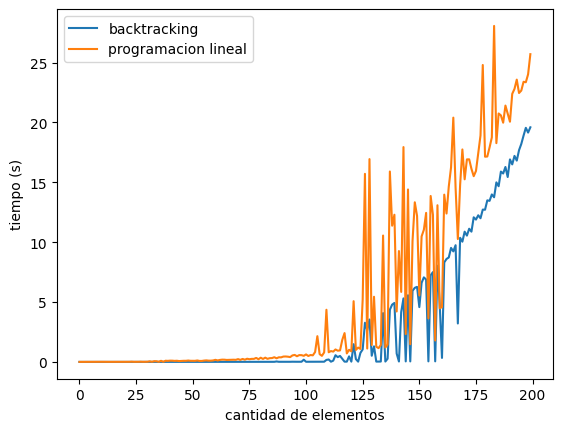
\includegraphics[width=1\textwidth]{img/backvslp.png}
\end{figure}

Backtracking obtiene mejores tiempo de ejecución que programación lineal para
encontrar la solución óptima.

\subsection{Algoritmos de aproximaci\'on}

\begin{figure}[H]
    \centering
    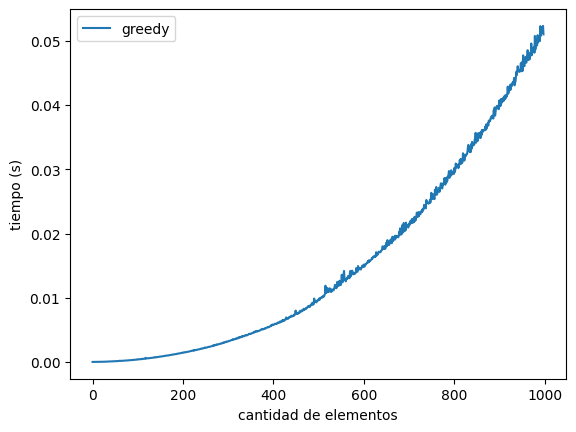
\includegraphics[width=0.49\textwidth]{img/greedy.png}
    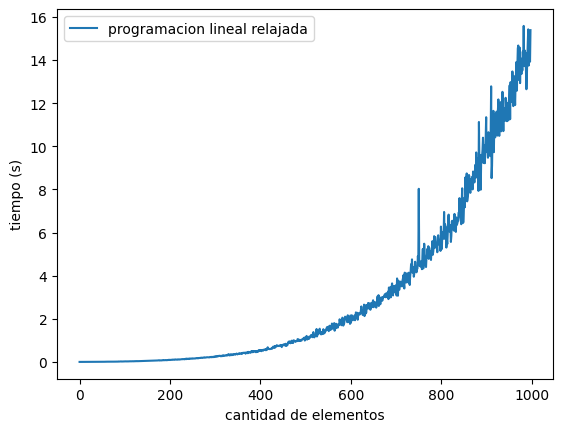
\includegraphics[width=0.49\textwidth]{img/pl_rlx.png}
\end{figure}

Notar la diferencia de tiempos (eje y) entre greedy y programación lineal.

\newpage
\section{Programación Lineal}

\subsection{Definiciones}

\subsubsection{Variables}

\begin{center}
    $Y_i$ := Variables binarias, indican si el elemento $A_{Y_i}$ forma parte
    de la solución. \\ (una por cada elemento en $A$)
\end{center}

\subsection{Modelo}

\subsubsection{Restricciones}

Necesitamos que haya por lo menos un elemento en cada subset, esto los
modelamos con una restricción por cada subset que toma la suma de las variables
asociadas a sus elementos y fuerza a esta a valer por lo menos uno:

\begin{equation}
    \sum_{Y \in B_i} Y \ge 1 \qquad \forall \quad B_i \in B
\end{equation}

\subsubsection{Funcional}

Estamos tratando de minimizar la cantidad de elementos en el resultado, por lo
que minimizamos el valor de la suma de las variables asociadas a los elementos
en el conjunto A.

\begin{equation}
    \min \{ \sum_{Y \in A} Y \}
\end{equation}

\subsection{Relajación}

Si dejamos que las variables $Y_i$ tomen valores reales el nuevo problema puede
ser resuelto en tiempo polinomial. Con esta solución podemos calcular una cota
inferior para el $k$ óptimo:

\begin{equation}
    \label{eq:k}
    k \ge \ceil{k_r} \qquad \text{con} \ k_r := \text{óptimo del problema
    relajado}
\end{equation}

Esto se debe a que al relajar las restricciones la solución solo puede mejorar.

Además, si tomamos las variables cuyo valor excede $\frac{1}{b}$, con $b =
\max_{B_i \in B}(|B_i|)$, obtenemos una solución aproximada. Esto es porque la
suma del valor de las variables de cada subset debe ser por lo menos 1, y hay a
lo sumo $b$ variables de cada subset, por lo que debe haber por lo menos una
variable en cada subset cuyo valor es mayor o igual a $\frac{1}{b}$, y al
utilizar todas las variables de valor mayor o igual a $\frac{1}{b}$ nos
aseguramos de tener por lo menos una variable de cada subset.

\subsubsection{Complejidad}

La complejidad del algoritmo con restricciones relajadas depende del algoritmo
utilizado por la librería \texttt{PuLP}. Si se utilizara el método simplex, si
bien es eficiente en la práctica tiene peor caso exponencial. Existen otros
algoritmos para resolver problemas de programación lineal que funcionan en
tiempo polinomial, como el algoritmo de Karmarkar.

\subsubsection{Calidad}

\[ \frac{A(I)}{z(I)} \le b \qquad \text{con} \ b := \max_{B_i \in B}(|B_i|) \]

\begin{proof}

    Aprovechamos la ecuación \eqref{eq:k} para obtener una cota inferior para
    $z(I)$:

    \[ k_r \le z(I) \]
    \[ k_r b \le z(I) b \]

    También sabemos que nuestra aproximación $A(I)$, define que las variables
    con valor mayor o igual a $\frac{1}{b}$ serán 1. En el peor caso, todas las
    variables valen $\frac{1}{b}$ y pasan a valer 1, lo que nos deja con una
    función objetivo a lo sumo $b$ veces peor:

    \[ A(I) \le k_r b \, \implies \, A(I) \le z(I) b \]

    Si definimos $r(A)$ tal que $\frac{A(I)}{z(I)} \le r(A)$ obtenemos $r(A) =
    b$.
\end{proof}

\newpage
\subsection{Algoritmo}

Para encontrar una soluci\'on aproximada al \textit{Hitting-Set Problem},
proponemos el siguiente algoritmo \textit{Greedy}:

\lstinputlisting[language=Python]{code/greedy.py}

\newpage
\section{Conclusiones}

Algunas cosas que caben destacar son los distintos usos que dimos o podr\'iamos
dar a los algoritmos de aproximaci\'on para disminuir el costo de encontrar la
soluci\'on \'optima, como la utilizaci\'on de la soluci\'on obtenida por el
algoritmo \textit{Greedy} como cota superior en la busqueda por
\textit{Backtracking}, y el valor del funcional al relajar las restricciones
del modelo lineal puede ahorrarnos una iteraci\'on si se utilizara como cota
inferior de $k$ (aunque esto solo funcionar\'ia si la soluci\'on es exactamente
$\ceil{k_r}$). El primero de estos mejor\'o el tiempo de ejecuci\'on de la
busqueda en un 10\%.



\newpage
\end{document}
